% Very simple template for lab reports. Most common packages are already included.
\documentclass[a4paper, 11pt]{article}
\usepackage[utf8]{inputenc} % Change according your file encoding
\usepackage{graphicx}
\usepackage{url}
\usepackage{float}

%opening
\title{Seminar Report\\Loggy - A logical time logger}
\author{Thomas FATTAL}
\date{\today{}}

\begin{document}

\maketitle

\section{Introduction}

In this exercise, we learnt how to use logical time in a concrete example: a message logger. A logging procedure receives messages from workers processes. All the messages are tagged with a Lamport timestamp. The goal of this experimentation was to display ordered messages on the logger side.


\section{Main problems and solutions}

That problem was a little tricky because we had to create the architecture which is able to order the received messages.\\
Finally, we used a queue that can contain the messages of the workers. The detailed architecture is presented on section 3.3.



\section{Evaluation}
\subsection{Chapter 3: Test}
If we run the method test:start() given in the third part, messages displayed are not ordered. Indeed, some "received" message are logged before "sending" message.

\begin{verbatim}
log : paul na {received,{hello,64}}			// Receive before sending message.
log : ringo na {sending,{hello,29}}
log : george na {sending,{hello,1}}
log : george na {received,{hello,29}}
log : john na {sending,{hello,64}}			// Here is the sending.
log : john na {received,{hello,1}}
log : george na {received,{hello,2}}
log : ringo na {sending,{hello,2}}
\end{verbatim}

Two reasons are available to explain this problem:
\begin{enumerate}
\item The logger process doesn't have a procedure to order messages yet. When the logger receives a message, it logs it immediately.
\item Because of the jitter, the "sending" message arrived after the "receiving" message.
\end{enumerate}

\subsection{Chapter 4: Lamport Time}
In this chapter, we added logical timestamp into the messages sent by the worker process. The timestamp is calculated according to Lamport theory by getting the max between the local time and the time of the received message, and by increasing by 1.
\begin{verbatim}
NewTime = erlang:max(CurrentCounter,Time)+1
\end{verbatim}
The console result is shown below:
\begin{verbatim}
log : paul 2 {received,{hello,64}} <-- Wrong order 
log : ringo 1 {sending,{hello,29}}
log : george 1 {sending,{hello,1}}
log : george 3 {received,{hello,29}}
log : john 1 {sending,{hello,64}} <-- Wrong order 
log : john 3 {received,{hello,1}}
\end{verbatim}

The messages are still in a wrong order, like the chapter 3 because we didn't improve the logger yet. However, by having logical time into the workers process, we ensure that the intra-process messages are ordered.

\subsection{Chapter 5: The tricky part}
To order the messages received by the logger, I decided to store received messages into a queue that looks like the following:

\begin{figure}[H]
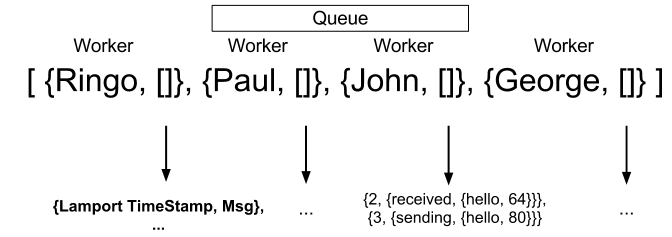
\includegraphics[scale=0.5]{archi_5.png}
\centering
\end{figure}

Each worker has a list of messages that contains the logical timestamp and the contents of the message.\\
When a message is received, it is saved into the list associated to the worker that sent the message. 

After, we look inside all the lists of workers. If all the list contain at least one message, we can display the first messages. We look at the message that have the smaller timestamp and we display it. After deleting it, we recurse into the function, until one of the worker has no messages waiting in the queue.\\

The logger works pretty well and the messages displayed are well ordered:

\begin{verbatim}
log : george 1 {sending,{hello,1}}
log : john 1 {sending,{hello,64}}
log : ringo 1 {sending,{hello,29}}
log : john 2 {received,{hello,1}}
log : george 2 {received,{hello,29}}
log : paul 2 {received,{hello,64}}
log : ringo 2 {sending,{hello,2}}
log : john 3 {sending,{hello,90}}
log : george 3 {received,{hello,2}}
log : paul 3 {sending,{hello,80}}
log : george 4 {sending,{hello,65}}
log : paul 4 {received,{hello,90}}
log : ringo 4 {received,{hello,80}}
\end{verbatim}

Some problems can appear:
\begin{itemize}
\item If a worker disconnects from the network, how to handle the disconnection? When a worker disconnects, he can send a message 'Down' to the logger. After that, the logger will remove the worker entry on the queue and the messages will continue to be displayed.
\item And if the message 'Down' is lost / If the worker doesn't send any 'Down' Message? We can set up a timeout. When the timeout is reached, the worker that has an empty list will be removed from the queue.
\end{itemize} 

\section{Conclusions}
With that exercise, we can see that, even concurrency is nice, it brings some problems compared to a single process system. Logical time answers very well to the question, by letting know the order of messages across time.\\

That exercise was very good to learn Erlang too and it's very interesting to see the progress that we did on Erlang language, just in three weeks.


\end{document}
